\chapter{PROBE: Isotropic Covariance Models through k-Nearest Neighbours}
\label{app:appendix_probe_knn}

\section{Introduction}

This appendix presents our initial exploratory work on isotropic covariance modelling for image features through k-nearest-neighbours. 
Unlike the work we presented in \Cref{ch:probe}, here we opt to learn a scalar weight, $\beta_i$, that represents the \textit{quality} of image features. We use $\beta_i$ to scale the covariance of each feature during non-linear optimization. 
We learn this quality ($\beta_i$) \textit{indirectly} by computing an egomotion estimate with a small subset of visual features and then storing the resulting position error in a prediction space. We repeat this for a fixed amount of iterations. During testing, we map features into this prediction space and compute a $\beta_i$ based on the $K$ nearest errors in this prediction space. Our framework is flexible enough that we do not require ground truth at every image and we can, potentially, learn the model based on a single loop closure error. 

\begin{remark}{Associated Publication}
This initial work is associated with the following publication:
\begin{itemize}
\item \bibentry{2015_Peretroukhin_PROBE}.	
\end{itemize}
\end{remark}

\section{Theory}

To solve for the relative egomotion, $\Transform_t$, between two camera frames, $\CoordinateFrame{c_0}$ and $\CoordinateFrame{c_1}$, we follow the technique described in \Cref{sec:vo_point_cloud} to convert stereo observations into point-clouds and then solve for the maximum likelihood $\LieGroupSE{3}$ transformation. We associate with each match $\{\ImageLandmark{i}{c_0}, \ImageLandmark{i}{c_1}\}$ a vector of
\emph{predictors}, $\Predictor{i}{t}$. We compute the covariance as a function of these predictors, so
that $\ImageLandmarkCovariance{i}{c_0} =\ImageLandmarkCovariance{i}{c_1} = \ImageLandmarkCovariance{i}{t} = \Covariance( \Predictor{i}{t})$, and we use the same covariance function for features in both frames\footnote{We conjecture that this is reasonable in a VO setup, where images change minimally between consecutive frames.},
\begin{align}
	\ImageLandmark{i}{c_0} &\sim \NormalDistribution\left(\bar{\Vector{y}}_{i,c_0}, \ImageLandmarkCovariance{i}{t} \right) = \NormalDistribution\left(\bar{\Vector{y}}_{i,c_0}, \Covariance( \Predictor{i}{t})\right) \\
		\ImageLandmark{i}{c_1}, &\sim \NormalDistribution\left(\bar{\Vector{y}}_{i,c_1}, \ImageLandmarkCovariance{i}{t} \right) = \NormalDistribution\left(\bar{\Vector{y}}_{i,c_1}, \Covariance( \Predictor{i}{t})\right).
\end{align}
This then builds the following weighted least squares objective,
\begin{equation}
  \Transform_t^* = \ArgMin{\Transform\in\text{SE}(3)}\sum_{i=1}^{N_t} 
  \Transpose{\Vector{e}_{i}(\Transform_t)} \GeneralCovariance_{i,t}^{-1} \Vector{e}_{i}(\Transform_t).
\end{equation}
where $\GeneralCovariance_{i,t}$ is now given by,
\begin{equation}
	\GeneralCovariance_{i,t} = \Matrix{D}\Matrix{G}_{i,c_1} \Covariance( \Predictor{i}{t})  \Matrix{G}_{i,c_1}^T \Matrix{D}^T + 
 \Matrix{D}\Transform_t \Matrix{G}_{i,c_0} \Covariance( \Predictor{i}{t}) \Matrix{G}_{i,c_0}^T  \Transform_t^T \Matrix{D}^T
\end{equation}
We build a model for $\Covariance( \Predictor{i}{t})$ as,
\begin{equation}
\Covariance( \Predictor{i}{c}) = \beta(\Predictor{i}{t}) \bar{\Covariance},
\end{equation}
with
\begin{equation}
 \beta(\Predictor{i}{c}) = \left(\frac{1}{\PROBEPoseError_\text{avg} K} \sum_{k=1}^K \PROBEPoseError_k  \right)^{\gamma}, ~ \PROBEPoseError_k \in \textsc{k-NN}(\Predictor{i}{t}),
\end{equation}

where $\{\PROBEPoseError_k\}_{k=1}^K$ are $K$ egomotion errors that are `nearest' to $\Predictor{i}{c}$, $\epsilon_\text{avg}$ is an average error, $\bar{\Covariance}$ is a baseline \textit{nominal} covariance, and $\gamma > 1$ is a hyper-parameter designed to exaggerate the effect of small changes in position error.

\section{Training}
Training proceeds by traversing the training path, selecting a subset of visual features at each step, and using them to compute an incremental position estimate. By comparing the estimated position to the ground truth position, we compute the translational Root Mean Squared Error (RMSE), $\epsilon$, and store it at each feature's position in the prediction space. The full algorithm is summarized in \Cref{alg:probe_train}. 
%\begin{figure}[h]
%\begin{center}
%\begin{algorithmic}[1]
%\Procedure{trainPROBE}{}
%\For{$l\gets 1, N_{iter}$}
%\For{$s\gets 1, N_{path}$}
%	\State $f_1, \dots, f_J \gets \text{samplefeatures}(l)$
%	\State $\mbs\pi^1_l, \dots, \mbs\pi^J_l \gets predictors(f_1, \dots, f_J)$
%	\State $\bar{\mbf{C}}_{ba},  \bar{\mbf{r}}_a^{ba} \gets poseChange(f_1, \dots, f_J)$
%	\State $\mbf \alpha_{l,s}  \gets computeRMSE(\bar{\mbf{r}}_a^{ba}, {\mbf{r}_{a}^{ba}}_{GT} )$
%	\State  $ \Theta_{l,s} \gets \left\{\mbs\pi^1_{l,s}, \dots, \mbs\pi^J_{l,s}, \alpha_{l,s}\right\}$
%\EndFor
%\EndFor
%\State \textbf{return} $\mbs \Theta = \{ \Theta_{l,s} \}$
%\EndProcedure
%\end{algorithmic}
%\caption{The PROBE training procedure.}\label{fig:ProbeTraining}
%\end{center}
%\end{figure}

\begin{algorithm}
  \caption{Train PROBE based on a dataset ($\mathcal{D}$) of pairs of input sensor data ($\mathcal{I}_s$) and ground truth egomotion ($\Transform_s$).}
   \label{alg:probe_train}
  \begin{algorithmic}
    \Function{BuildPROBEModel}{$\mathcal{D}$}
      \For{$l \gets [1,...,N_{iter}]$}
      \ForAll{$\mathcal{I}_s$, $\Transform_s$ in $\mathcal{D}$}
	\State $\mathcal{F} \gets$ \Call{extractFeatures}{$\mathcal{I}_s$}
	\State $\{f_1, \dots, f_J\} \gets$ \Call{sample}{$\mathcal{F}$}
	\State $\Estimate{\Transform} \gets$ \Call{computeTransform}{$\{f_1, \dots, f_J\}$}
	\State $\mbf \PROBEPoseError  \gets$ \Call{error}{$\Estimate{\Transform}, \Transform_s$}
	\State $\{\Predictor{s}{1}, \dots, \Predictor{s}{J}\} \gets$ \Call{predictor}{$\{f_1, \dots, f_J\}$}
	\State Insert $\{\Predictor{s}{1}, \dots,  \Predictor{s}{J}\}$ into $\mathcal{M}$ and store $\PROBEPoseError$ at all $J$ locations
	\EndFor
      \EndFor
      \State\Return  $\mathcal{M}$
    \EndFunction
  \end{algorithmic}
\end{algorithm}

\section{Testing}
To use the PROBE model in a test environment, we compute the location of each observed visual feature in our prediction space, and then compute its relative weight $\beta_i$ as a function of its $K$ nearest neighbours in the training set.
For efficiency, the $K$ nearest neighbours are found using a $k$-d tree.
The final scaling factor $\beta_i$ is a function of the mean of the $\alpha$ values corresponding to the $K$ nearest neighbours, normalized by $\PROBEPoseError_\text{avg}$, the mean $\alpha$ value of the entire training set.

\begin{algorithm}
  \caption{Compute scalar covariance factors, $\beta_i$, for a set of stereo feature tracks (and IMU data), $\mathcal{F}$, given a PROBE model $\mathcal{M}$.}
  \label{alg:probe_test}
  \begin{algorithmic}
    \Function{UsePROBE}{$\mathcal{M}$, $\mathcal{F}, \gamma$}
     \State $\PROBEPoseError_\text{avg} \gets$ \Call{averageError}{$\mathcal{M}$}
      \ForAll{$f_i$ in $\mathcal{F}$}
        \State $\Vector{\phi}_i \gets$ \Call{predictor}{$f_i$} 
        \State $\PROBEPoseError_1,...,\PROBEPoseError_K \gets$ \Call{findKNN}{$\Vector{\phi}_i, K, \mathcal{M}$}
		\State $\beta_i \gets \left(\frac{1}{\PROBEPoseError_\text{avg} K} \sum_{k=1}^K \PROBEPoseError_k  \right)^{\gamma}$
		
	   \EndFor
      \State\Return $\mbs \beta = \{\beta_i\}$
    \EndFunction
  \end{algorithmic}
\end{algorithm}


The value of $K$ can be determined through cross-validation, and in practice depends on the size of the training set and the environment.
The computation of $\beta_i$ is designed to map small differences in learned $\alpha$ values to scalar weights that span several orders of magnitude.
An appropriate value of $\gamma$ can be found by searching through a set range of candidate values and choosing the value that minimizes the average RMSE (ARMSE) on the training set.

\begin{figure}
    \centering
    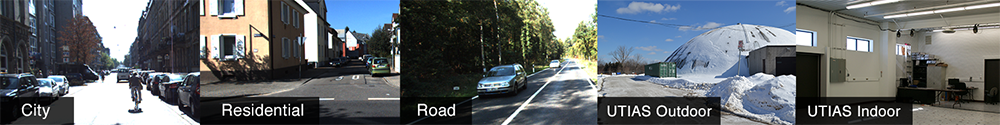
\includegraphics[width=\textwidth]{probe/city-res-road.png}
    \caption{Three types of environments in the KITTI dataset, as well as 2 types of environments at the University of Toronto.  We use one trial from each category to train and then evaluate separate trials in the same category.}
    \label{fig:probe_KITTI-Types}
\end{figure}

\section{Experiments}
We trained and evaluated this version of PROBE in two sets of experiments.
The first set of experiments made use of 4.5 km of data from the City, Residential, and Road categories of the KITTI dataset \citep{Geiger2013-ky}.
In the second set of experiments, we collected indoor and outdoor datasets at the University of Toronto Institute for Aerospace Studies (UTIAS) using a Skybotix VI-Sensor mounted on an Adept MobileRobots Pioneer 3-AT rover and a Clearpath Husky rover, respectively (\Cref{fig:probe_huskypic}).
In both cases, the camera recorded stereo images at 10 Hz while the IMU operated at 200 Hz.
The outdoor dataset consisted of a 264 m training run followed by a 302 m evaluation run, with ground truth provided by RTK-corrected GPS.
The indoor dataset consisted of a 32 m training run and a 33 m evaluation run through a room with varying lighting and shadows.
For the indoor dataset, no ground truth was available, so we trained PROBE using only the knowledge that the training path should form a closed loop.

\begin{figure}
    \centering
    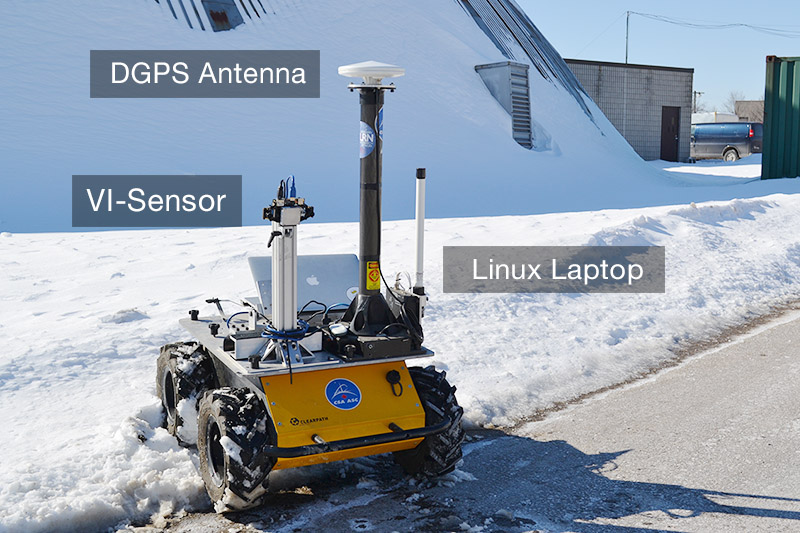
\includegraphics[width=0.6\textwidth]{probe/husky2}
    \caption{Our four-wheeled skid-steered Clearpath Husky rover equipped with Skybotix VI-Sensor and Ashtech DGPS antenna used to collect the outdoor UTIAS dataset.}
    \label{fig:probe_huskypic}
\end{figure}

We compare PROBE to what we call a \textit{nominal} visual-inertial navigation pipeline (or VINS, a pipeline based on the point-cloud-error-based VO described in \Cref{ch:vo}, but with an initial estimate of rotation given by integrating angular velocities from an IMU), as well as a VINS with an aggressive RANSAC routine. In the nominal pipeline, we use RANSAC with enough iterations to be 99\% confident that we select only inliers when as many as 50\% of the features are outliers. In the aggressive case, we increase the confidence level to 99.99\%. When PROBE is used, we apply a pre-processing step that makes use of the rotational estimate from the IMU to reject any egregious feature matches by thresholding the cosine distance between pairs of matched feature vectors. We assume small translations between frames and typically set the threshold to reject feature vectors that are separated by more than five degrees. 

For feature extraction, matching, and sparse optical flow calculations, we use the open source vision library \textsf{viso2} \citep{Geiger2011-xe}.
For all prediction space calculations, we use features in the left image of the stereo pair.

To evaluate PROBE, we run a nominal VINS pipeline on a given test trial, tune the RANSAC threshold to achieve reasonable translation error ($< 5\%$ final drift), then repeat the trial with the aggressive RANSAC procedure. Finally, we run this procedure again, this time disabling RANSAC completely and applying our trained PROBE model (with pre-processing) to each observed feature.  \Cref{table:probe_kitti_data} compares the performance of each trained PROBE model to that of the nominal VINS pipeline and aggressive-RANSAC VINS.

\begin{table}
    \centering
    
    \caption{Comparison of translational Average Root Mean Square Error (ARMSE) and Final Translational Error on the KITTI dataset.}
	\resizebox{\columnwidth}{!}{%
    % Need to add an asterisk to the 30_drive_0027 "Type" to indicate that it's trained on City data, but can't do it without messing up the justification - Matt
    \begin{threeparttable}
        \begin{tabular}{cccccccccccc}
        & & & & \multicolumn{2}{c}{Nominal RANSAC} & & \multicolumn{2}{c}{Aggressive RANSAC} & & &  \\
        	 & & & & \multicolumn{2}{c}{(99\% outlier rejection)} & & \multicolumn{2}{c}{(99.99\% outlier rejection)} & & \multicolumn{2}{c}{PROBE} \B \\
             \cline{5-6} \cline{8-9} \cline{11-12}
        	 Trial & Type & Path Length &&  ARMSE & Final Error & & ARMSE & Final Error & & ARMSE & Final Error \T\B \\ \hline \T
        	\texttt{26\_drive\_0051} & City \tnote{1} & 251.1 m && 4.84 m & 12.6 m && 3.30 m & 8.62 m && 3.48 m & 8.07 m \\
        	\texttt{26\_drive\_0104} & City \tnote{1} & 245.1 m && 0.977 m & 4.43 m && 0.850 m & 3.46 m && 1.19 m & 3.61 m \\ 
        	\texttt{29\_drive\_0071} & City \tnote{1} & 234.0 m && 5.44 m & 30.3 m && 5.44 m & 30.4 m && 3.03 m & 12.8 m \\ 
        		\texttt{26\_drive\_0117} & City \tnote{1} & 322.5 m && 2.29 m & 9.07 m && 2.29 m & 9.07 m && 2.76 m & 9.08 m \\ 
        		\texttt{30\_drive\_0027} & Residential \tnote{1, \dag} & 667.8 m && 4.22 m & 12.2 m && 4.30 m & 10.6 m && 3.64 m & 4.57 m \\ 
        		\texttt{26\_drive\_0022} & Residential \tnote{2} & 515.3 m && 2.21 m & 3.99 m && 2.66 m & 6.09 m && 3.06 m & 4.99 m \\ 
        		\texttt{26\_drive\_0023} & Residential \tnote{2} & 410.8 m && 1.64 m & 8.20 m && 1.77 m & 8.27 m && 1.71 m & 8.13 m \\ 
        		\texttt{26\_drive\_0027} & Road \tnote{3} & 339.9 m && 1.63 m & 8.75 m && 1.63 m & 8.65 m && 1.40 m & 7.57 m \\ 
        		\texttt{26\_drive\_0028} & Road \tnote{3} & 777.5 m && 4.31 m & 16.9 m && 3.72 m & 13.1 m && 3.92 m & 13.2 m \\ 
        		\texttt{30\_drive\_0016} & Road \tnote{3} & 405.0 m && 4.56 m & 19.5 m && 3.33 m & 14.6 m && 2.76 m & 13.9 m \\ 
                UTIAS Outdoor & Snowy parking lot & 302.0 m && 7.24 m & 10.1 m && 7.02 m & 10.6 m && 6.85 m & 6.09 m \\ 
                UTIAS Indoor & Lab interior & 32.83 m && --- & 0.854 m && --- & 0.738 m && --- & 0.617 m  \B \\    
        \hline
            \label{table:probe_kitti_data}
        \end{tabular}
        \begin{tablenotes}
            \item[1] Trained using sequence \texttt{09\_26\_drive\_0005}. ~$^2$ Trained using sequence  \texttt{09\_26\_drive\_0046}. ~$^3$ Trained using sequence  \texttt{09\_26\_drive\_0015}.  
            \item[\dag] This residential trial was evaluated with a model trained on a sequence from the city category because of several moving vehicles that were better represented in that training dataset.
        \end{tablenotes}
    \end{threeparttable}
    }
\end{table}

